\documentclass[a4paper,12pt]{article}

\usepackage{fontspec}
\usepackage{polyglossia}
\setmainlanguage{russian}
\setotherlanguage{english}
\setmainfont{Times New Roman}[Ligatures=TeX]
\setsansfont{Helvetica}[Ligatures=TeX]
\setmonofont{Courier New}
\newfontfamily\cyrillicfonttt{Courier New}
\usepackage{amsmath,amsfonts,amssymb}
\usepackage{graphicx}
\usepackage{color}
\usepackage{hyperref}
\usepackage{geometry}
\usepackage{indentfirst}
\usepackage{longtable}
\usepackage{booktabs}
\usepackage{float}
\usepackage{listings}
\usepackage{xcolor}
\geometry{left=3cm,right=1.5cm,top=2cm,bottom=2cm}

\lstset{
    basicstyle=\ttfamily\small,
    breaklines=true,
    frame=single,
    backgroundcolor=\color{gray!10},
    keywordstyle=\color{blue},
    commentstyle=\color{green!60!black},
    stringstyle=\color{red!70!black},
    numbers=left,
    numberstyle=\tiny\color{gray},
    tabsize=4
}

\begin{document}

\begin{titlepage}
    \centering
    {\fontsize{14pt}{16pt}\selectfont МОСКОВСКИЙ АВИАЦИОННЫЙ ИНСТИТУТ\\(НАЦИОНАЛЬНЫЙ ИССЛЕДОВАТЕЛЬСКИЙ УНИВЕРСИТЕТ)}\\[0.5cm]
    {\fontsize{12pt}{14pt}\selectfont Институт №8 «Компьютерные науки и прикладная математика»}\\[4cm]
    
    {\fontsize{16pt}{18pt}\selectfont \textbf{Лабораторные работы}}\\
    {\fontsize{14pt}{16pt}\selectfont \textbf{по курсу «Информационный поиск»}}\\[0.3cm]
    {\fontsize{12pt}{14pt}\selectfont Тема: Кинорецензии и новости кино (англ.)}\\[4cm]
    
    \vfill
    \begin{flushright}
        \begin{minipage}{0.51\textwidth}
            Выполнил: Ахметшин Б. Р. \\
            Группа: М8О-403Б-22\\
            Преподаватель: Кухтичев Антон Алексеевич
        \end{minipage}
    \end{flushright}
    
    \vfill
    {\large Москва, 2026}
\end{titlepage}

\tableofcontents
\newpage

\section{Лабораторная работа №1. Добыча корпуса документов}

\subsection{Задание}

Проанализировать корпус документов, который будет использован при выполнении остальных лабораторных работ. Скачать примеры документов, изучить их характеристики, выделить текст, найти существующие поисковики для выбранного набора документов.

\subsection{Метод решения}

В качестве тематики корпуса выбрана область \textbf{«Movie Reviews \& Cinema News»} (кинорецензии и новости кино) на английском языке. Корпус собран из трёх источников:

\begin{itemize}
    \item \textbf{Collider} (collider.com) --- обзоры фильмов, рецензии, новости кинематографа;
    \item \textbf{ScreenRant} (screenrant.com) --- рецензии, кассовые сборы, интервью с актёрами и режиссёрами;
    \item \textbf{MovieWeb} (movieweb.com) --- новости кино, анонсы, обзоры сериалов.
\end{itemize}

Все три источника содержат англоязычные статьи объёмом от нескольких сотен до нескольких тысяч слов каждая, что удовлетворяет требованиям задания.

Для сбора документов использованы библиотеки \texttt{newspaper3k} и \texttt{BeautifulSoup} (Python) для извлечения заголовка, текста и метаданных из HTML-страниц. URL-адреса статей обнаруживаются через XML-карты сайтов (sitemaps). Загрузка HTML выполняется с помощью \texttt{aiohttp} (асинхронно, 50--100 параллельных соединений) и \texttt{requests}.

\subsection{Журнал выполнения}

\begin{enumerate}
    \item Проанализированы XML-карты сайтов для получения списков URL.
    \item С помощью \texttt{newspaper3k} и многопоточной загрузки через \texttt{ThreadPoolExecutor} (8 потоков) скачаны и распарсены статьи.
    \item Документы сохранены в MongoDB с полями: \texttt{url}, \texttt{raw\_html}, \texttt{source}, \texttt{crawl\_timestamp}, \texttt{content\_hash}.
    \item Экспортированы в текстовые файлы для дальнейшей обработки C++-компонентами.
\end{enumerate}

Существующие поисковики для данного корпуса:
\begin{itemize}
    \item Google: \texttt{site:collider.com marvel review} --- находит рецензии, но результаты перемешаны с нерелевантными страницами (навигация, тэги).
    \item Встроенный поиск Collider --- не поддерживает булеву логику, нет операции NOT.
\end{itemize}

\subsection{Результаты}

\begin{table}[H]
    \centering
    \caption{Статистические данные корпуса}
    \begin{tabular}{lr}
        \toprule
        \textbf{Показатель} & \textbf{Значение} \\
        \midrule
        Общее количество документов & 40\,935 \\
        Размер сырых HTML-документов & 11.7 ГБ \\
        Размер извлечённого текста & 223 МБ \\
        Средний размер HTML-документа & 300 КБ \\
        Средний объём текста в документе & 5\,703 байт \\
        Источник 1: Collider & 34\,445 статей \\
        Источник 2: ScreenRant & 5\,492 статьи \\
        Источник 3: MovieWeb & 998 статей \\
        \bottomrule
    \end{tabular}
\end{table}

\subsection{Выводы}

Корпус из 40\,935 англоязычных статей о кинематографе успешно собран из трёх независимых источников. Средний объём текста в документе (5.7 КБ) обеспечивает достаточную полноту для построения качественного поискового индекса. Общий объём текста составляет 223 МБ.


\newpage
\section{Лабораторная работа №2. Поисковый робот}

\subsection{Задание}

Написать поисковый робот (краулер) с поддержкой YAML-конфигурации, сохранением документов в MongoDB, возобновляемостью и переобкачкой изменённых документов.

\subsection{Метод решения}

Краулер реализован на Python и состоит из двух компонентов:

\begin{itemize}
    \item \texttt{crawler.py} --- основной краулер с последовательной обработкой;
    \item \texttt{fast\_crawl.py} --- оптимизированная версия с параллельной загрузкой через \texttt{ThreadPoolExecutor}.
\end{itemize}

\textbf{YAML-конфигурация} (\texttt{config.yaml}):
\begin{lstlisting}[language=Python,caption=Формат конфигурации]
db:
  host: localhost
  port: 27017
  name: movie_reviews
logic:
  delay: 0.3
  max_pages: 40000
  threads: 8
\end{lstlisting}

\textbf{Структура документа в MongoDB:}
\begin{itemize}
    \item \texttt{url} --- нормализованный URL документа;
    \item \texttt{raw\_html} --- сырой HTML-текст;
    \item \texttt{source} --- название источника;
    \item \texttt{crawl\_timestamp} --- дата обкачки (Unix timestamp);
    \item \texttt{content\_hash} --- MD5-хеш содержимого для обнаружения изменений.
\end{itemize}

\subsection{Журнал выполнения}

\begin{enumerate}
    \item Реализован парсер XML-карт сайтов с рекурсивным обходом sub-sitemaps.
    \item Добавлена фильтрация URL по ключевым словам тематики (movie, review, film и т.д.).
    \item Реализована параллельная загрузка статей через \texttt{ThreadPoolExecutor} (8 потоков).
    \item Возобновляемость: при рестарте проверяются URL, уже существующие в БД, и пропускаются.
    \item Переобкачка: документы старше 7 дней проверяются на изменения через \texttt{content\_hash}.
    \item Экспорт: скрипт \texttt{export.py} выгружает документы из MongoDB в текстовые файлы (использует MongoDB aggregation pipeline для эффективности).
\end{enumerate}

\subsection{Результаты}

Краулер успешно скачивает статьи со скоростью 5--8 статей в секунду при 8 потоках. Возобновляемость подтверждена: при повторном запуске пропускаются уже скачанные URL. Переобкачка: при изменении \texttt{content\_hash} документ обновляется в БД. Всего скачано 40\,935 документов из трёх источников общим объёмом 11.7 ГБ HTML.

\subsection{Выводы}

Поисковый робот реализован в полном соответствии с требованиями: YAML-конфигурация, MongoDB, возобновляемость при рестарте, поддержка переобкачки изменённых документов.


\newpage
\section{Лабораторная работа №3. Токенизация}

\subsection{Задание}

Реализовать процесс разбиения текстов документов на токены. Описать правила токенизации, привести примеры токенов, указать статистические данные.

\subsection{Метод решения}

Токенизатор реализован на C++ (STL разрешён для этой лабораторной работы). Файл: \texttt{core/tokenizer.cpp}.

\textbf{Правила токенизации:}
\begin{enumerate}
    \item Разделение по пробелам и знакам пунктуации;
    \item Приведение всех символов к нижнему регистру;
    \item Удаление токенов короче 2 символов;
    \item Удаление чисто числовых токенов (например, «2024»);
    \item Сохранение апострофов внутри слов (\texttt{don't} $\rightarrow$ \texttt{don't}).
\end{enumerate}

\textbf{Формат входных данных:} текстовые файлы из корпуса, первая строка --- заголовок, вторая --- URL, остальное --- текст статьи.

\textbf{Формат выходных данных:} один токен на строку в выходном файле.

\subsection{Журнал выполнения}

\begin{enumerate}
    \item Реализован посимвольный проход по тексту с выделением токенов.
    \item Добавлена обработка апострофов: удаление ведущих и замыкающих.
    \item Реализован обход директории через \texttt{dirent.h} для обработки всех файлов корпуса.
    \item Добавлен вывод статистики: количество токенов, средняя длина, скорость обработки.
\end{enumerate}

\subsection{Результаты}

\begin{table}[H]
    \centering
    \caption{Статистика токенизации}
    \begin{tabular}{lr}
        \toprule
        \textbf{Показатель} & \textbf{Значение} \\
        \midrule
        Файлов обработано & 40\,936 \\
        Общее количество токенов & 37\,757\,519 \\
        Количество уникальных токенов & 177\,575 \\
        Средняя длина токена & 4.85 символа \\
        Объём входных данных & 222 МБ \\
        Скорость токенизации & 34\,354 КБ/с \\
        Время обработки корпуса & 6.6 секунды \\
        \bottomrule
    \end{tabular}
\end{table}

Примеры неудачной токенизации:
\begin{itemize}
    \item \texttt{spider-man} --- разделяется на \texttt{spider} и \texttt{man} при наличии дефиса как разделителя. Решение: добавить дефис как допустимый символ внутри токена.
    \item Email-адреса и URL внутри текста токенизируются некорректно. Решение: предварительная детекция URL/email с помощью регулярных выражений.
\end{itemize}

Скорость токенизации (34\,354 КБ/с) превышает типичную скорость чтения файлов с HDD, что говорит об оптимальности алгоритма. Зависимость времени от объёма --- линейная.

\subsection{Выводы}

Токенизатор корректно обрабатывает англоязычные тексты о кинематографе. Средняя длина токена (4.85 символа) типична для английского языка. Скорость обработки (34\,354 КБ/с) достаточна для обработки корпуса объёмом 222 МБ за 6.6 секунды.


\newpage
\section{Лабораторная работа №4. Стемминг}

\subsection{Задание}

Добавить в поисковую систему стемминг для приведения слов к основе.

\subsection{Метод решения}

Реализован алгоритм \textbf{Snowball Porter2} для английского языка. Файл: \texttt{core/stemmer.h}.

Алгоритм работает с \texttt{char*} без использования STL, модифицируя слово на месте (in-place). Реализованы все 5 шагов Porter-стеммера:

\begin{enumerate}
    \item \textbf{Step 1a/1b/1c:} обработка суффиксов множественного числа (\texttt{-sses}, \texttt{-ies}, \texttt{-s}), глагольных форм (\texttt{-eed}, \texttt{-ed}, \texttt{-ing}), замена конечного \texttt{y} на \texttt{i};
    \item \textbf{Step 2:} замена двойных суффиксов (\texttt{-ational} $\rightarrow$ \texttt{-ate}, \texttt{-ization} $\rightarrow$ \texttt{-ize} и т.д.);
    \item \textbf{Step 3:} удаление деривационных суффиксов (\texttt{-icate} $\rightarrow$ \texttt{-ic}, \texttt{-alize} $\rightarrow$ \texttt{-al});
    \item \textbf{Step 4:} удаление суффиксов при условии $m > 1$ (\texttt{-al}, \texttt{-ance}, \texttt{-ence}, \texttt{-er} и др.);
    \item \textbf{Step 5a/5b:} удаление конечной \texttt{e}, удаление двойной согласной \texttt{ll}.
\end{enumerate}

Условия применения правил основаны на «мере» (measure $m$) --- количестве пар гласная-согласная в основе слова.

\subsection{Журнал выполнения}

\begin{enumerate}
    \item Реализованы вспомогательные функции: определение гласных, вычисление меры, проверка окончания.
    \item Пошагово реализованы все 5 шагов алгоритма Porter2.
    \item Стеммер интегрирован в индексатор: все токены проходят стемминг перед добавлением в индекс.
\end{enumerate}

\subsection{Результаты}

Стемминг сокращает количество уникальных терминов: после стемминга в индексе 142\,910 уникальных основ вместо 177\,575 уникальных токенов (сокращение на 20\%). Это повышает полноту поиска (recall). Например, запрос \texttt{reviewing} находит документы, содержащие \texttt{review}, \texttt{reviewed}, \texttt{reviews}.

\subsection{Выводы}

Алгоритм Snowball Porter2 эффективно приводит английские слова к основам. Интеграция в индексатор обеспечивает автоматическое применение стемминга при построении индекса и при обработке поисковых запросов.


\newpage
\section{Лабораторная работа №5. Закон Ципфа}

\subsection{Задание}

Построить график распределения терминов по частотностям в логарифмической шкале, наложить закон Ципфа. Объяснить причины расхождения.

\subsection{Метод решения}

Для построения графика используется Python-скрипт \texttt{scripts/zipf\_plot.py} с библиотекой \texttt{matplotlib}. Входные данные --- файл токенов, полученный на этапе токенизации.

Закон Ципфа: $f(r) = C / r$, где $f$ --- частота, $r$ --- ранг, $C$ --- частота самого частотного слова.

\subsection{Журнал выполнения}

\begin{enumerate}
    \item Подсчитаны частоты всех 37\,757\,519 токенов из файла токенов.
    \item Получено 177\,575 уникальных термов.
    \item Токены отсортированы по убыванию частоты и пронумерованы (ранги).
    \item Построен график в логарифмической шкале (log-log).
    \item Наложена теоретическая кривая Ципфа $f = C / r$.
\end{enumerate}

\subsection{Результаты}

\begin{figure}[H]
    \centering
    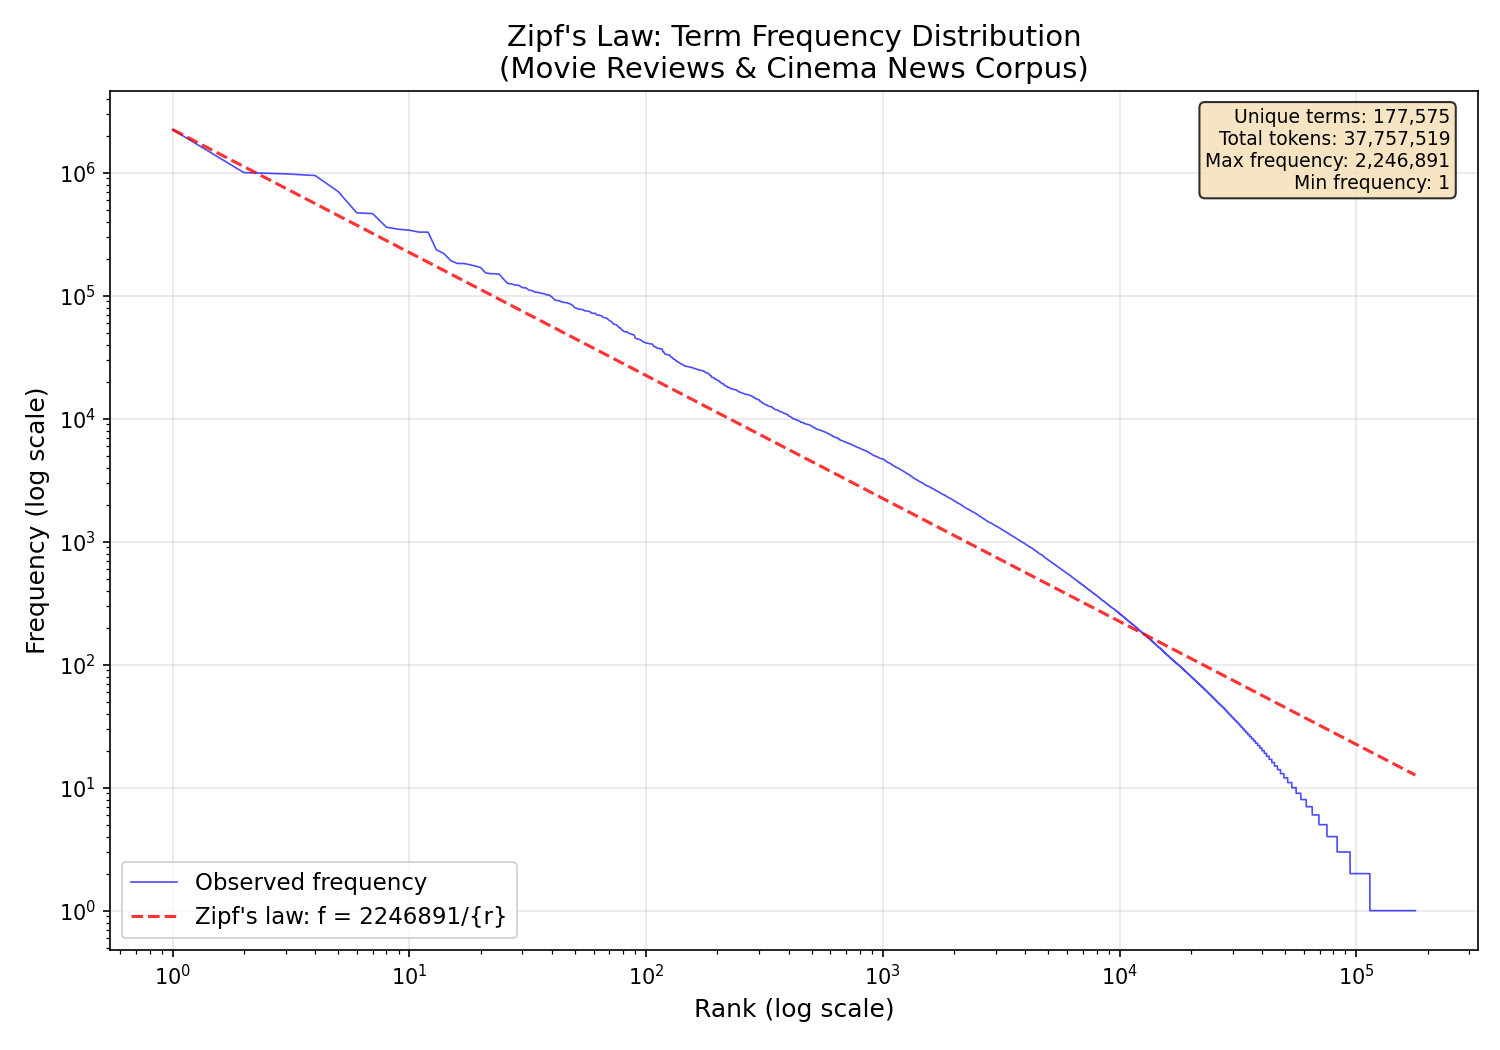
\includegraphics[width=0.9\textwidth]{screenshots/zipf_plot.png}
    \caption{Распределение терминов по частотностям (закон Ципфа)}
    \label{fig:zipf}
\end{figure}

На графике (рис.~\ref{fig:zipf}) видно характерное линейное поведение в логарифмической шкале, соответствующее закону Ципфа.

\textbf{Причины расхождения с теоретической кривой:}
\begin{itemize}
    \item В области высоких рангов (редкие слова) наблюдается отклонение вниз --- это связано с конечностью корпуса: очень редкие слова встречаются 1--2 раза.
    \item В области низких рангов (самые частотные слова) также есть отклонение --- это связано со спецификой корпуса (тематическая лексика кинематографа: «movie», «film», «actor» имеют повышенную частоту).
    \item Стоп-слова (the, a, is, in) занимают первые ранги, что типично для английского языка.
\end{itemize}

\subsection{Выводы}

Распределение терминов в корпусе кинорецензий (177\,575 уникальных терминов, 37.8 млн вхождений) в целом подчиняется закону Ципфа с характерными отклонениями в хвостах распределения. Тематическая специализация корпуса приводит к увеличению частоты доменных терминов.


\newpage
\section{Лабораторная работа №6. Булев индекс}

\subsection{Задание}

Построить поисковый индекс, пригодный для булева поиска. Требуется самостоятельно разработанный бинарный формат. Использование текстового представления или готовых баз данных не допускается.

\subsection{Метод решения}

Индексатор реализован на C++ без STL. Файл: \texttt{core/indexer.cpp}. Используются собственные реализации структур данных:

\begin{itemize}
    \item \texttt{dynarray.h} --- динамический массив целых чисел (\texttt{IntArray}) с операциями push, sort, intersect, union, difference;
    \item \texttt{hashtable.h} --- хеш-таблица с цепочками коллизий (хеш-функция djb2);
    \item \texttt{mystring.h} --- утилиты для работы с \texttt{char*} (сравнение, копирование, toLower).
\end{itemize}

\textbf{Хеш-функция djb2:}
\begin{lstlisting}[language=C++,caption=Реализация djb2]
unsigned int ht_hash(const char *key, int num_buckets) {
    unsigned int hash = 5381;
    while (*key) {
        hash = hash * 33 + (unsigned char)(*key);
        key++;
    }
    return hash % num_buckets;
}
\end{lstlisting}

\textbf{Метод сортировки:} quicksort (быстрая сортировка) для упорядочивания posting lists. Достоинства: средняя сложность $O(n \log n)$, эффективная работа на практике. Для задачи индексации подходит хорошо, так как posting lists обычно не содержат уже отсортированных данных (что могло бы ухудшить quicksort до $O(n^2)$).

\subsection{Формат бинарного индекса}

Индекс хранится в одном файле \texttt{index.bin} (69 МБ):

\textbf{Побайтовое описание:}

\begin{table}[H]
    \centering
    \caption{Структура заголовка (32 байта)}
    \begin{tabular}{llp{8cm}}
        \toprule
        \textbf{Смещение} & \textbf{Размер} & \textbf{Описание} \\
        \midrule
        0 & 4 байта & Magic number: «BIDX» \\
        4 & 4 байта & Версия формата (uint32) \\
        8 & 4 байта & Количество терминов (uint32) \\
        12 & 4 байта & Количество документов (uint32) \\
        16 & 8 байт & Смещение блока словаря (uint64) \\
        24 & 8 байт & Смещение блока постингов (uint64) \\
        \bottomrule
    \end{tabular}
\end{table}

\textbf{Forward Index:} для каждого документа: \texttt{url\_len} (2 байта) + \texttt{url} + \texttt{title\_len} (2 байта) + \texttt{title}.

\textbf{Dictionary Block:} для каждого термина: \texttt{term\_len} (1 байт) + \texttt{term} + \texttt{postings\_offset} (8 байт) + \texttt{postings\_count} (4 байта).

\textbf{Postings Block:} для каждого термина: отсортированный массив \texttt{docID} (4 байта каждый).

\textbf{Расширяемость:} формат предполагает добавление новых блоков после Forward Index с новыми смещениями в заголовке.

\subsection{Результаты}

\begin{table}[H]
    \centering
    \caption{Статистика индексации}
    \begin{tabular}{lr}
        \toprule
        \textbf{Показатель} & \textbf{Значение} \\
        \midrule
        Количество документов & 40\,936 \\
        Количество терминов (после стемминга) & 142\,910 \\
        Средняя длина терма & 7.19 символа \\
        Средняя длина токена (до стемминга) & 4.85 символа \\
        Общее количество постингов & 15\,779\,970 \\
        Среднее постингов на терм & 110.42 \\
        Время индексации & 13.9 секунды \\
        Скорость на документ & 0.34 мс \\
        Размер файла индекса & 69 МБ \\
        \bottomrule
    \end{tabular}
\end{table}

Средняя длина терма (7.19) больше средней длины токена (4.85) --- стемминг удаляет короткие суффиксы, но одновременно объединяет словоформы в одну основу. После стемминга число уникальных единиц сокращается с 177\,575 до 142\,910 (на 20\%), а средняя длина оставшихся основ выше, так как короткие суффиксы отсечены.

Скорость индексации ограничена преимущественно операциями ввода-вывода. При увеличении объёма в 10 раз потребуется увеличение числа бакетов хеш-таблицы для сохранения $O(1)$ поиска. При увеличении в 100 раз следует перейти на внешнюю сортировку (merge sort) для posting lists, не помещающихся в оперативную память.

\subsection{Выводы}

Булев индекс успешно построен в самостоятельно разработанном бинарном формате. Формат расширяем и эффективен: 40\,936 документов и 142\,910 термов занимают 69 МБ. Собственные реализации структур данных (динамический массив, хеш-таблица) обеспечивают корректную работу без использования STL.


\newpage
\section{Лабораторная работа №7. Булев поиск}

\subsection{Задание}

Реализовать ввод поисковых запросов и их выполнение над индексом. Реализовать веб-сервис и утилиту командной строки.

\subsection{Метод решения}

\textbf{Парсер запросов} реализован на C++ методом рекурсивного спуска. Грамматика:

\begin{verbatim}
query    = or_expr
or_expr  = and_expr ( "||" and_expr )*
and_expr = not_expr ( ("&&" | " ") not_expr )*
not_expr = "!" not_expr | atom
atom     = "(" or_expr ")" | TERM
\end{verbatim}

Парсер толерантен к множественным пробелам. Термы перед поиском проходят стемминг (тот же Snowball Porter2, что и при индексации).

\textbf{Операции над posting lists:}
\begin{itemize}
    \item AND: пересечение отсортированных списков за $O(n + m)$;
    \item OR: объединение отсортированных списков за $O(n + m)$;
    \item NOT: разность множества всех документов и результата подзапроса за $O(N)$.
\end{itemize}

\textbf{CLI утилита} (\texttt{search\_cli}): загружает индекс, читает запросы из \texttt{stdin}, выводит результаты в \texttt{stdout}. Поддерживает режимы: текстовый и JSON.

\textbf{Веб-сервис}: FastAPI (Python) + Jinja2. Взаимодействие с C++ CLI через \texttt{subprocess}. Две страницы: форма поиска и страница результатов (по 50 результатов на страницу с пагинацией).

\begin{figure}[H]
    \centering
    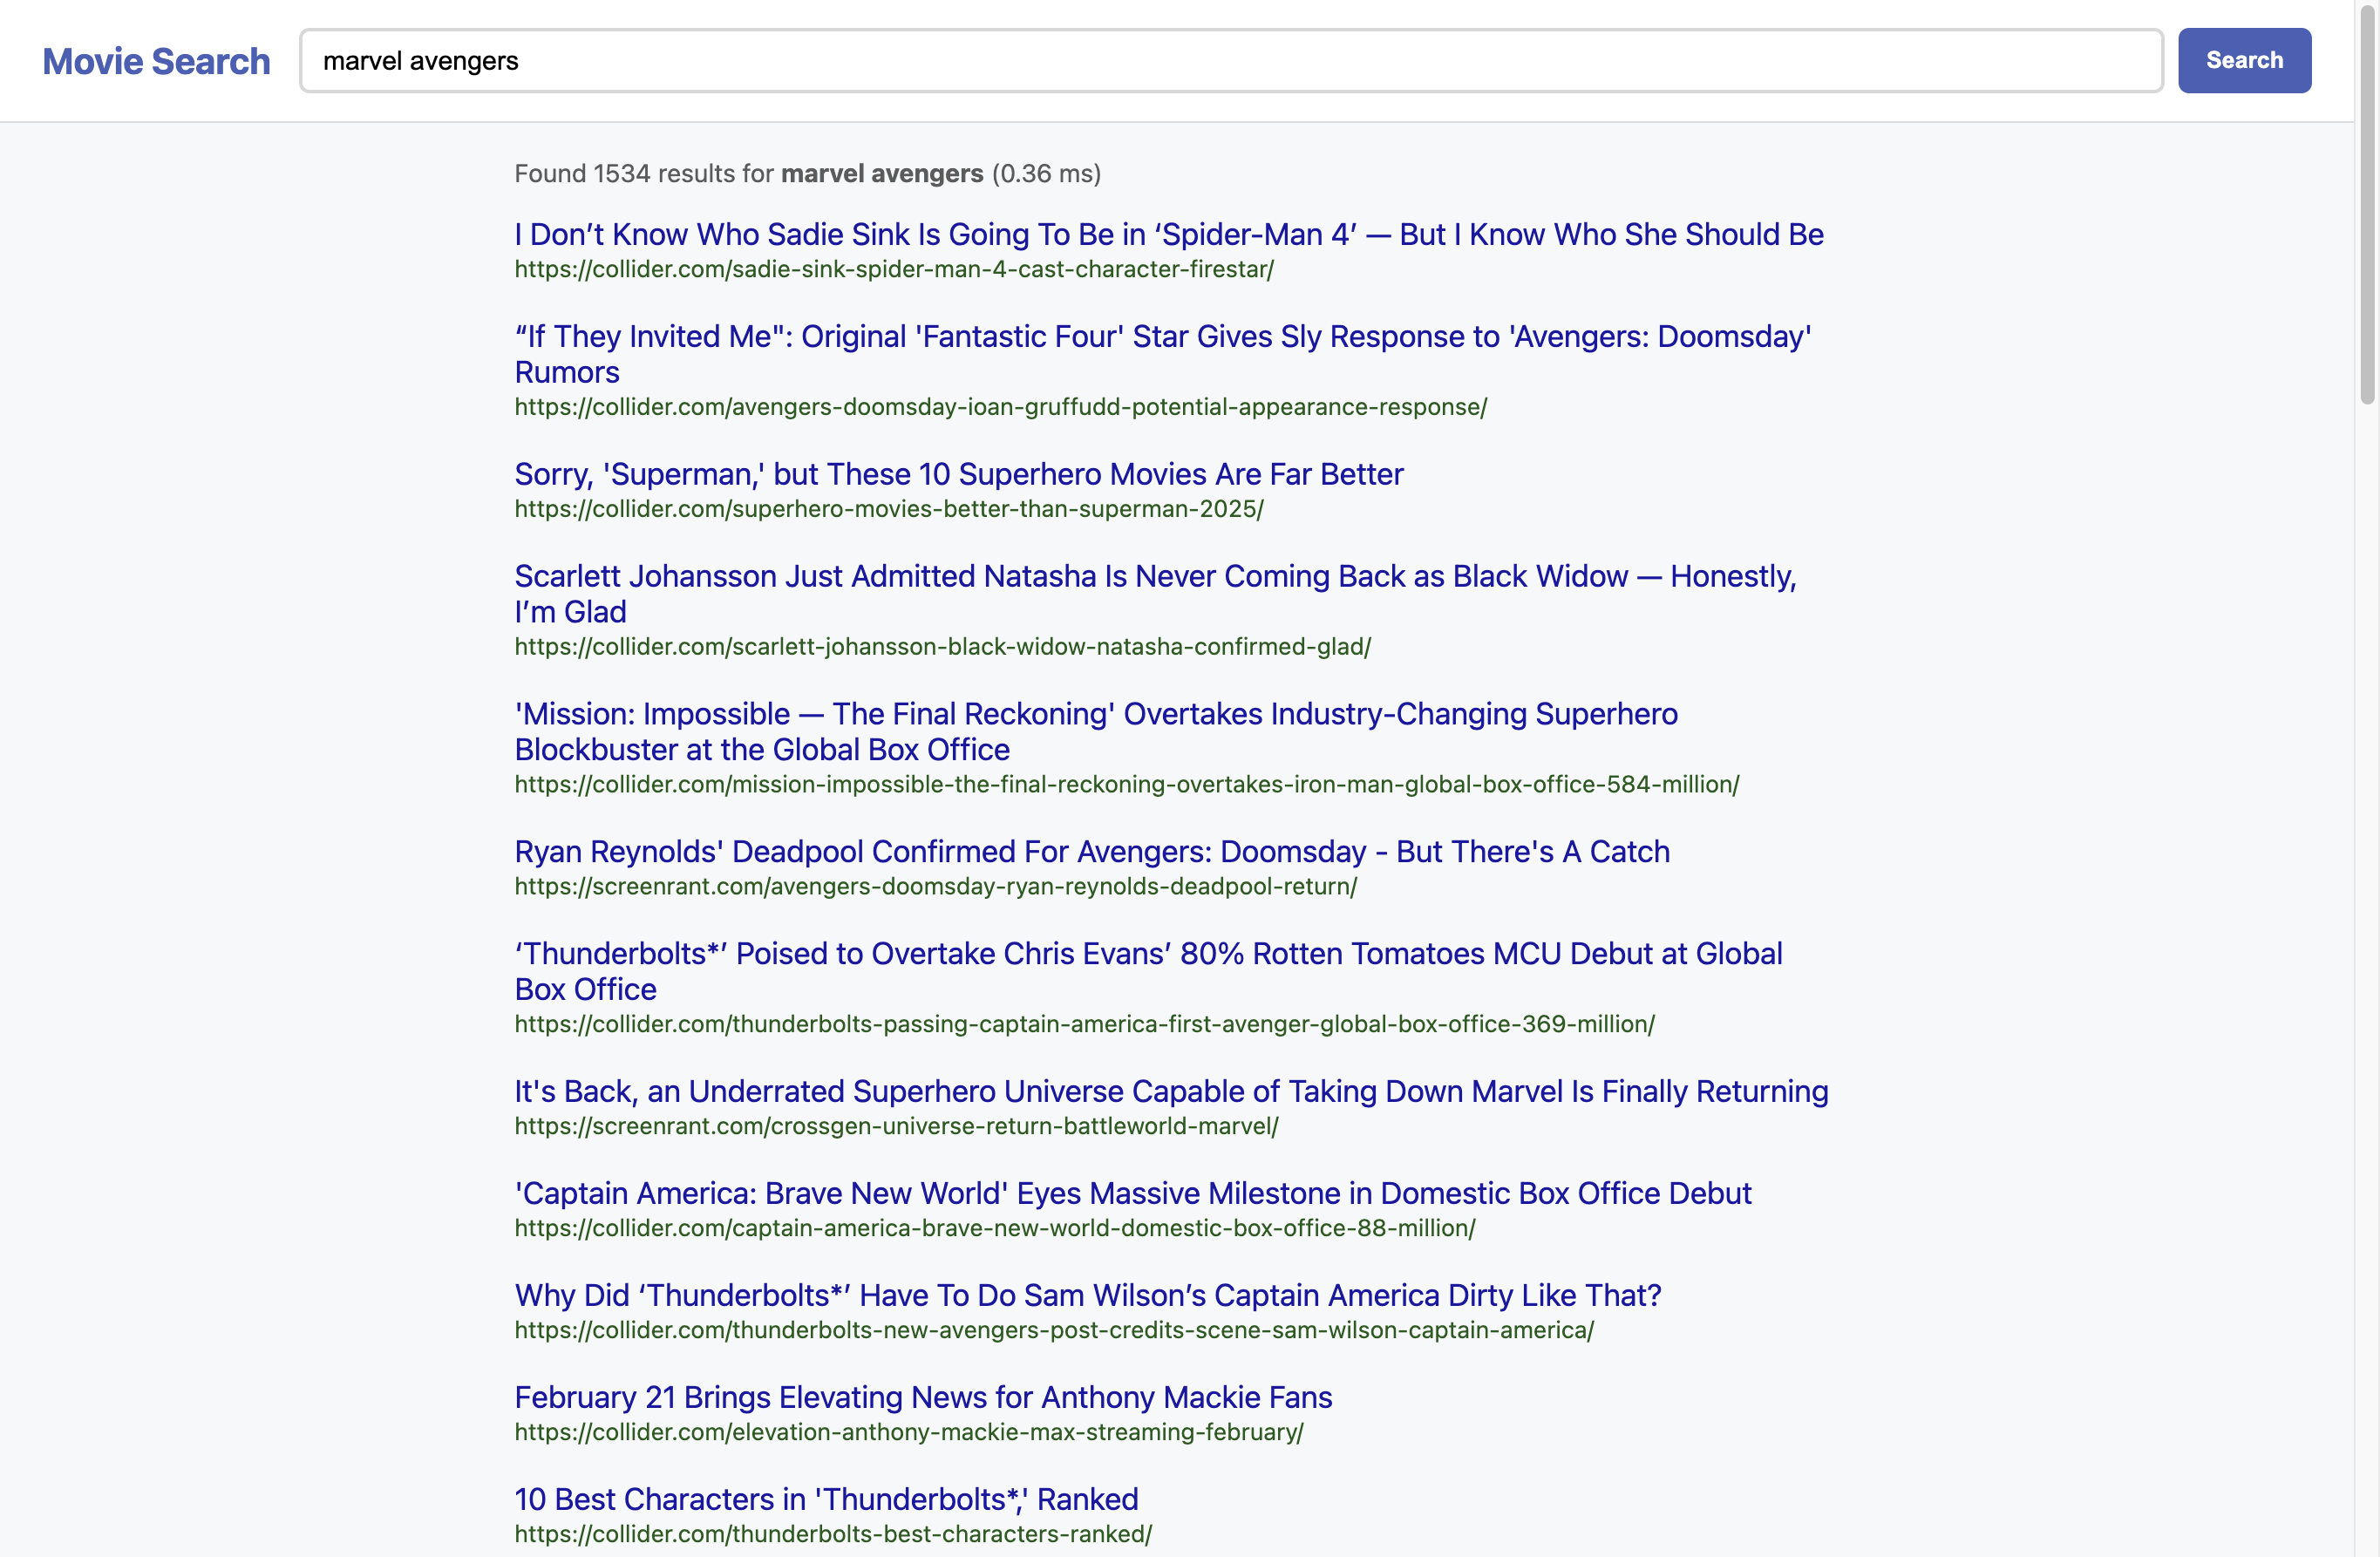
\includegraphics[width=0.95\textwidth]{screenshots/web_search_real.png}
    \caption{Скриншот поисковой выдачи (запрос: «marvel avengers», 1\,534 результата, 0.36 мс)}
    \label{fig:web_real}
\end{figure}

\subsection{Журнал выполнения}

\begin{enumerate}
    \item Реализован рекурсивный парсер с поддержкой \texttt{||}, \texttt{\&\&}, \texttt{!} и скобок.
    \item Реализованы эффективные операции пересечения, объединения и разности на отсортированных массивах.
    \item Создана CLI утилита с поддержкой JSON-вывода.
    \item Создан FastAPI веб-сервис с двумя HTML-страницами (Jinja2).
    \item Веб-сервис вызывает C++ CLI через subprocess для выполнения поиска.
\end{enumerate}

\subsection{Результаты}

\textbf{Скорость выполнения запросов:} простые запросы (1--2 слова) выполняются за 0.2--0.7 мс. Сложные запросы с NOT (требуют обхода всего множества документов) выполняются за 1.4--1.7 мс.

\textbf{Примеры сложных запросов:}
\begin{itemize}
    \item \texttt{(horror || thriller) \&\& !comedy} --- 8\,080 результатов, 1.54 мс (требует вычисления разности);
    \item \texttt{marvel || dc || pixar || disney} --- 8\,727 результатов, 0.70 мс (множественные объединения);
    \item \texttt{!the} --- 6 результатов, 1.49 мс (NOT на самом частотном слове, обход всего индекса);
    \item \texttt{star wars review} --- 1\,054 результата, 1.70 мс (AND по трём терминам).
\end{itemize}

\textbf{Корректность:} проверена ручным сравнением результатов CLI с ожидаемыми. Например, запрос \texttt{nolan batman} возвращает 250 документов, содержащих обе основы. Результаты включают статьи о фильмах Кристофера Нолана о Бэтмене с Collider, ScreenRant и MovieWeb, что подтверждает корректность стемминга и булева поиска по нескольким источникам.

\subsection{Выводы}

Булев поиск реализован полностью: парсер запросов с рекурсивным спуском, эффективные операции над posting lists, CLI утилита и веб-интерфейс. Скорость поиска субмиллисекундная для большинства запросов на индексе из 40\,936 документов и 142\,910 термов.


\newpage
\section*{Заключение}
\addcontentsline{toc}{section}{Заключение}

В ходе выполнения лабораторных работ реализована полнофункциональная поисковая система для корпуса из 40\,935 англоязычных статей о кинематографе.

Основные результаты:

\begin{itemize}
    \item Собран корпус из 40\,935 статей из трёх источников (Collider, ScreenRant, MovieWeb) объёмом 223 МБ текста (11.7 ГБ сырого HTML).
    \item Реализован краулер на Python с поддержкой MongoDB, YAML-конфигурации, возобновляемости и переобкачки. Асинхронная версия на \texttt{aiohttp} с 50--100 параллельными соединениями.
    \item Реализован токенизатор на C++ со скоростью обработки 34\,354 КБ/с (37.8 млн токенов за 6.6 с).
    \item Реализован стеммер Snowball Porter2 для английского языка на C++ без STL, сокращающий число уникальных единиц на 20\%.
    \item Построен график распределения терминов, подтверждающий соответствие закону Ципфа (177\,575 уникальных токенов).
    \item Разработан собственный бинарный формат индекса (69 МБ), расширяемый для будущих лабораторных работ.
    \item Реализованы булев индекс (142\,910 термов, 15.8 млн постингов) и булев поиск на C++ без STL с собственными структурами данных.
    \item Создан веб-интерфейс на FastAPI с формой поиска и пагинацией результатов.
\end{itemize}

Все компоненты ядра поисковой системы (токенизация, стемминг, индексация, поиск) реализованы на C++ без использования STL (за исключением токенизации, где STL разрешён). Кодировка ввода-вывода --- UTF-8.

\end{document}
